\documentclass[11pt,a4paper]{article}

% ---- Packages ----
\usepackage[margin=2.5cm]{geometry}
\usepackage{graphicx}
\usepackage{listings}
\usepackage{xcolor}
\usepackage{hyperref}
\usepackage{booktabs}
\usepackage{amsmath}
\usepackage{amssymb}
\usepackage{enumitem}
\usepackage{float}
\usepackage{caption}
\usepackage{subcaption}
\usepackage{tikz}
\usetikzlibrary{shapes.geometric, arrows.meta, positioning, fit}

% ---- Code listing style ----
\lstset{
    language=Python,
    basicstyle=\ttfamily\small,
    keywordstyle=\color{blue}\bfseries,
    commentstyle=\color{gray},
    stringstyle=\color{red!70!black},
    numbers=left,
    numberstyle=\tiny\color{gray},
    numbersep=5pt,
    frame=single,
    breaklines=true,
    captionpos=b,
    tabsize=4,
    showstringspaces=false
}

% ---- Title ----
\title{
    \vspace{-1cm}
    \textbf{CE/CZ4123/SC4023 Big Data Management} \\[0.3cm]
    \large Semester Group Project Report \\[0.2cm]
    \large HDB Resale Flat Column-Store Query Engine
}
\author{
    % TODO: Fill in your group members' names and matriculation numbers
    Pham Ba Cong (Matriculation No.: U2331760J) \\
    Aylin Stecher (Matriculation No.: N2500024C) \\
    abc (Matriculation No.:)
}
\date{}

\begin{document}
\maketitle
\thispagestyle{empty}

% =============================================================
\section{Data Storage}
% =============================================================

\subsection{Column-Store Architecture}

Our program implements a column-oriented storage engine from scratch in Python, without relying on external libraries such as pandas or SQL databases. In contrast to row-oriented storage where each record is stored as a contiguous unit, our \texttt{ColumnStore} class stores each attribute as an independent array. This layout provides two key advantages for analytical queries: (1)~only the columns relevant to a query are accessed, avoiding unnecessary I/O on irrelevant fields, and (2)~iterating over a single column array is cache-friendly since values are contiguous in memory.

Figure~\ref{fig:row-vs-col} illustrates the difference. When computing \texttt{MIN(price\_per\_sqm)} with a filter on \texttt{town}, the column store only touches the \texttt{town} and \texttt{price\_per\_sqm} arrays, while a row store would load all 10+ fields per row.

\begin{figure}[H]
\centering
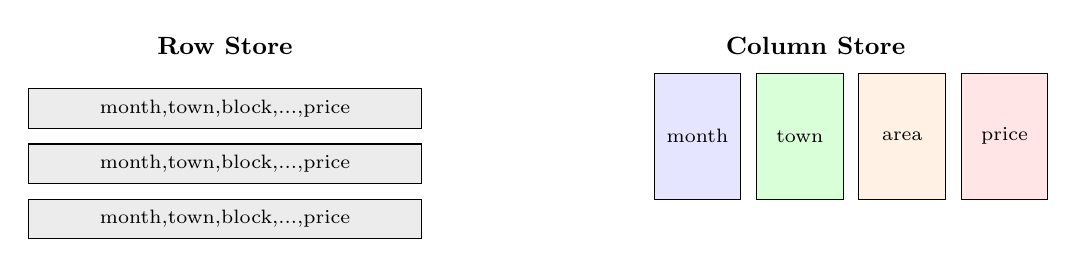
\begin{tikzpicture}[
    colbox/.style={draw, minimum width=1.2cm, minimum height=0.5cm, font=\scriptsize},
    arrw/.style={-{Stealth}, thick}
]
% Row store
\node[font=\small\bfseries] at (0, 1.8) {Row Store};
\foreach \i/\data in {0/{month,town,block,...,price}, 1/{month,town,block,...,price}, 2/{month,town,block,...,price}} {
    \node[colbox, minimum width=5cm, fill=gray!15] at (0, 1.0-\i*0.7) {\data};
}
% Column store
\node[font=\small\bfseries] at (7.5, 1.8) {Column Store};
\foreach \j/\col/\clr in {0/month/blue!10, 1/town/green!15, 2/area/orange!10, 3/price/red!10} {
    \node[colbox, minimum width=1.1cm, minimum height=1.6cm, fill=\clr] at (6.0+\j*1.3, 0.65) {\col};
}
\end{tikzpicture}
\caption{Row-oriented vs.\ column-oriented storage layout. Our implementation uses the column layout (right), where each attribute is stored as an independent array.}
\label{fig:row-vs-col}
\end{figure}

\subsection{Dictionary Encoding for String Columns}

String columns such as \texttt{town}, \texttt{flat\_type}, and \texttt{flat\_model} contain many repeated values. Storing and comparing raw strings is both memory-intensive and slow. Our \texttt{Dictionary} class implements \emph{dictionary encoding}: each unique string is assigned a sequential integer code, and the column array stores only these codes.

\begin{lstlisting}[caption={Dictionary encoding example}, label={lst:dict}]
d = Dictionary()
d.encode("BEDOK")      # -> 0
d.encode("CLEMENTI")   # -> 1
d.encode("BEDOK")      # -> 0 (already encoded)
d.get_code("UNKNOWN")  # -> -1 (not found)
\end{lstlisting}

This yields two benefits: (a)~filtering by \texttt{town == "BEDOK"} becomes an integer comparison (\texttt{col[i] == 0}), which is significantly faster; (b)~memory usage is reduced since each row stores a 4-byte integer rather than a variable-length string. The dataset contains 26 distinct towns and 7 flat types, making dictionary encoding highly effective.

\subsection{Schema Definition and Derived Columns}

We define an explicit schema for the HDB dataset mapping each column name to its type (\texttt{"int"}, \texttt{"float"}, or \texttt{"str"}). This avoids the overhead of per-row type inference during loading. After the initial load, we add three \emph{derived columns} computed from the raw data:

\begin{itemize}[nosep]
    \item \texttt{year} (int) --- parsed from \texttt{month} (e.g., \texttt{"2020-06"} $\to$ 2020)
    \item \texttt{month\_num} (int) --- parsed from \texttt{month} (e.g., \texttt{"2020-06"} $\to$ 6)
    \item \texttt{price\_per\_sqm} (float) --- computed as \texttt{resale\_price / floor\_area\_sqm}
\end{itemize}

These derived columns are stored as first-class columns in the \texttt{ColumnStore}, enabling the query engine to filter and aggregate on them without re-computing values.

\subsection{File I/O}

The CSV is read using Python's built-in \texttt{csv} module. We optimized ingestion by using direct per-column appends instead of a per-row dictionary path, reducing the full-load time from 4.24\,s to 2.73\,s (1.55$\times$ faster). String values are dictionary-encoded on the fly. For output, we use \emph{late materialization}: string decoding via the dictionary is performed only for the result rows being written, not for the entire dataset.

\subsection{Exception Handling}

The program handles edge cases including: (a)~malformed CSV rows (rows with fewer columns than the header are skipped); (b)~values not present in the dictionary (the \texttt{get\_code} method returns $-1$, and the query immediately returns an empty result); (c)~empty query results (the output reports ``No result'' when no valid $(x, y)$ pairs are found and aggregation methods return \texttt{None}).


% =============================================================
\section{Data Processing}
% =============================================================

\subsection{Query Condition Derivation}

Query conditions are derived from the matriculation number via the \texttt{parse\_matric()} function:

\begin{itemize}[nosep]
    \item \textbf{Target year}: last digit $d$; if $d \geq 5$ then $2010 + d$, else $2020 + d$.
    \item \textbf{Start month}: second-to-last digit; 0 maps to October (10).
    \item \textbf{Towns}: all unique digits mapped through a lookup table (Table~\ref{tab:towns}).
\end{itemize}

For \texttt{U2331760J}: target year = 2020, start month = June (06), matched towns = BEDOK, BUKIT PANJANG, CLEMENTI, CHOA CHU KANG, PASIR RIS, TAMPINES.

\begin{table}[H]
\centering
\small
\begin{tabular}{c|cccccccccc}
\toprule
Digit & 0 & 1 & 2 & 3 & 4 & 5 & 6 & 7 & 8 & 9 \\
\midrule
Town & BDK & BKP & CLM & CCK & HGN & JRW & PSR & TPN & WDL & YSH \\
\bottomrule
\end{tabular}
\caption{Digit-to-town mapping (abbreviated). BDK=BEDOK, BKP=BUKIT PANJANG, CLM=CLEMENTI, CCK=CHOA CHU KANG, HGN=HOUGANG, JRW=JURONG WEST, PSR=PASIR RIS, TPN=TAMPINES, WDL=WOODLANDS, YSH=YISHUN.}
\label{tab:towns}
\end{table}

\subsection{Column-at-a-Time Filtering}

Our \texttt{Query} class applies filter predicates one column at a time. For each predicate, only the relevant column array is iterated---no full-row reconstruction is needed. The surviving row indices are progressively narrowed through successive predicates:

\begin{lstlisting}[caption={Chainable query API usage}]
row_idx, min_val = (store.query()
    .filter("year", "==", target_year)
    .filter("month_num", ">=", start_month)
    .filter("month_num", "<=", month_end)
    .filter("town", "in", matched_towns)
    .filter("floor_area_sqm", ">=", y)
    .min("price_per_sqm"))
\end{lstlisting}

For string columns, the \texttt{filter} method resolves human-readable values to dictionary codes before comparison. For example, \texttt{.filter("town", "in", ["BEDOK", "CLEMENTI"])} internally becomes an integer set membership test, which is substantially faster than comparing strings.

\subsection{Naive Baseline (\texttt{run\_query\_naive})}

The naive implementation issues an independent query for every $(x, y)$ pair ($8 \times 71 = 568$ queries). Each query re-scans the full dataset through the \texttt{Query} API. While correct and simple, this approach performs significant redundant work since queries for adjacent $(x, y)$ pairs overlap heavily.

\subsection{Optimized Query (\texttt{run\_query})}

The optimized implementation eliminates redundancy through two techniques:

\paragraph{Optimization 1: Incremental Month Accumulation.}
Instead of re-filtering from scratch for each $x$ value, we pre-filter all rows matching the target year and matched towns, then group them by month. As $x$ increases from 1 to 8, we only add the new month's rows to an accumulator:

\begin{itemize}[nosep]
    \item $x = 1$: candidates from month \texttt{start\_month}
    \item $x = 2$: reuse $x = 1$ candidates + add month \texttt{start\_month + 1}
    \item $x = k$: reuse $x = k{-}1$ candidates + add month \texttt{start\_month + k - 1}
\end{itemize}

We maintain a \texttt{best\_price\_at\_area[a]} array that tracks the minimum \texttt{price\_per\_sqm} seen for each exact floor area value. When a new month is added, only the new month's rows update this array.

\paragraph{Optimization 2: Area Sweep with Running Minimum.}
For a given $x$, the query asks: for each $y$, what is $\min(\text{price\_per\_sqm})$ where $\text{area} \geq y$? Since the condition $\text{area} \geq y$ includes all areas from $y$ up to the maximum, we perform a single backward sweep from \texttt{max\_area} down to \texttt{y\_min}, maintaining a running minimum. This answers all 71 values of $y$ in $O(\text{max\_area})$ time, rather than the $O(n \times 71)$ time of the naive approach.

\subsection{Vectorized Out-of-Core Loading}
\label{sec:vectorized}

For scenarios where the dataset may not fit in memory, we use a batch-oriented scan similar in spirit to vectorized execution in systems such as MonetDB and Vertica. The routine \texttt{iter\_load\_vectors} reads the CSV in fixed-size batches (default 4,096 rows) and builds a separate \texttt{ColumnStore} for each batch. The loader itself does \emph{not} filter rows or push predicates into the CSV scan---every batch is loaded in full, then processed.

For each batch, we run the same pipeline as the full-load path in \texttt{main.py}: derived columns (\texttt{post\_load\_transform}), sorted physical layout, zone maps, and the optimized \texttt{run\_query} from the previous subsection. Filters on \texttt{year}, \texttt{town}, and the $(x,y)$ sweep therefore use the same column-at-a-time \texttt{Query} implementation as Mode~1, but only over the rows currently resident in memory.

Batches partition the rows: the minimum \texttt{price\_per\_sqm} for a given $(x,y)$ in one batch might not be globally minimal. After each batch query, we merge partial results by retaining, for each $(x,y)$, whichever row has the lower \texttt{price\_per\_sqm} across batches seen so far (materializing the winning row for output). Working set stays bounded by roughly one batch plus this merge state, whereas the full-load path holds the entire table. Quantitative comparison of total time and query-stage peak memory appears in Table~\ref{tab:vec}.

\subsection{Late Materialization}

Throughout the pipeline, rows are represented as indices into column arrays. Full row reconstruction (including string decoding) is deferred until the final output stage via \texttt{materialize\_row()}. This avoids the cost of decoding dictionary-encoded strings for the thousands of rows that are ultimately filtered out.

\subsection{Storage and Query Optimizations}

We implemented two additional column-store optimizations to improve query performance.

\paragraph{Sorted Column Layout.}
All columns are physically sorted by \texttt{(year, month\_num, town)} via \texttt{sort\_by()}. This clusters records by the most common filter predicates. When combined with zone maps (below), sorted layout enables the zone map to skip entire contiguous regions of irrelevant data with high precision.

\paragraph{Zone Maps (Min-Max Indexes).}
For each block of 4,096 rows, we store the minimum and maximum value of key columns (\texttt{year}, \texttt{month\_num}, \texttt{town}, \texttt{floor\_area\_sqm}). Before scanning any block, the query engine checks whether the block's min-max range overlaps the filter predicate. Non-overlapping blocks are skipped entirely. Zone maps produced the largest single-optimization speedup: the optimized query dropped from 0.769\,s to 0.063\,s ($\mathbf{12.2\times}$ faster), and peak memory from 10.07\,MiB to 1.28\,MiB ($\mathbf{7.9\times}$ lower).

Table~\ref{tab:optim} presents the isolated and combined impact of each optimization.

\begin{table}[H]
\centering
\small
\setlength{\tabcolsep}{4pt}
\begin{tabular}{l r r r}
\toprule
\textbf{Config} & \textbf{Opt. query} & \textbf{Naive query} & \textbf{Opt. query peak mem} \\
\midrule
Baseline (none)             & 0.769\,s & 16.379\,s & 10.07\,MiB \\
Sorted layout only          & 0.616\,s & 15.239\,s & 10.07\,MiB \\
Zone maps only              & \textbf{0.063\,s} & 1.465\,s & \textbf{1.28\,MiB} \\
Full all (sort+zonemap)     & \textbf{0.063\,s} & \textbf{1.454\,s} & \textbf{1.28\,MiB} \\
\bottomrule
\end{tabular}
\caption{Isolated and combined impact of each optimization (10-run averages). Zone maps dominate: $12.2\times$ faster optimized queries vs.\ baseline, while sorting adds little once zone maps are enabled.}
\label{tab:optim}
\end{table}

\subsection{Performance Comparison}

Table~\ref{tab:perf} compares the full-load execution modes (10-run averages, sorted layout + zone maps enabled).

\begin{table}[H]
\centering
\begin{tabular}{l r r r r}
\toprule
\textbf{Mode} & \textbf{Load (s)} & \textbf{Query (s)} & \textbf{Total (s)} & \textbf{Peak mem} \\
\midrule
Full Load + Naive Query     & 3.864 & 1.454 & 5.318 & 1.28\,MiB \\
Full Load + Optimized Query & 3.864 & 0.063 & 3.927 & 1.28\,MiB \\
\bottomrule
\end{tabular}
\caption{Full-load execution modes (10-run averages, sorted layout + zone maps enabled). The optimized query is $23.1\times$ faster than naive at the query stage.}
\label{tab:perf}
\end{table}

\subsection{Vectorized Mode Comparison}

Table~\ref{tab:vec} benchmarks the chunked pipeline from Section~\ref{sec:vectorized} (4,096-row batches, same transform/layout/\texttt{run\_query} as full load, merged $(x,y)$ minima) against the full-load optimized query.

\begin{table}[H]
\centering
\begin{tabular}{l r r}
\toprule
\textbf{Mode} & \textbf{Total time (s)} & \textbf{Query peak mem} \\
\midrule
Full Load + Optimized Query & 3.927 & 1.28\,MiB \\
Vectorized Load + Query     & 5.296 & 0.18\,MiB \\
\midrule
Vectorized overhead         & $1.35\times$ slower & $7.1\times$ lower \\
\bottomrule
\end{tabular}
\caption{Vectorized mode vs.\ full-load optimized query (10-run averages, sorted layout + zone maps enabled, vector size = 4,096 rows). Query peak memory is measured for the query stage only. Vectorized mode runs the pipeline per vector and merges results, which adds repeated per-vector transform/layout/query work and control overhead.}
\label{tab:vec}
\end{table}

Vectorized mode is slower here because the workload fits in memory and the full-load path applies transform/layout once over the entire dataset. Chunking repeats these steps for each vector and adds merge overhead.


% =============================================================
\section{Experiment Result}
% =============================================================

\subsection{Execution Output}

We executed the program using matriculation number \texttt{U2331760J}. The derived query parameters are:
\begin{itemize}[nosep]
    \item Target year: 2020, start month: June (06)
    \item Matched towns: BEDOK, BUKIT PANJANG, CLEMENTI, CHOA CHU KANG, PASIR RIS, TAMPINES
    \item $x \in [1, 8]$, $y \in [80, 150]$, threshold: 4725
    \item Input rows loaded: 259,237
\end{itemize}

The program successfully executed all three query modes. Selected output metrics:
\begin{itemize}[nosep]
    \item Example MIN query: \texttt{CHOA CHU KANG, Block 295, 118\,sqm, \$325,000, price/sqm = 2754.24}
    \item Records in 2020 for matched towns: 6,532
    \item Average resale price in BEDOK (2020): \$411,303
    \item Mode~1 (optimized): \textbf{568} valid $(x, y)$ pairs, query time $0.063 \pm 0.002$\,s, peak 1.28\,MiB
    \item Mode~2 (naive): \textbf{568} valid $(x, y)$ pairs, query time $1.454 \pm 0.067$\,s
    \item Mode~3 (vectorized): \textbf{568} valid $(x, y)$ pairs, total time $5.296 \pm 0.118$\,s, query peak (max over chunks) $0.18$\,MiB
\end{itemize}

All three modes consistently report 568 valid $(x, y)$ pairs across all benchmark runs, and the naive/optimized verification result is \texttt{MATCH} in every run.

% TODO: Replace with actual screenshot of program execution
\begin{figure}[H]
\centering
\fbox{\parbox{0.9\textwidth}{\centering\vspace{2cm}\texttt{TODO: Insert screenshot of terminal output showing successful execution}\vspace{2cm}}}
\caption{Screenshot of program execution showing configuration, query results, and timing summary.}
\label{fig:exec}
\end{figure}

\subsection{Output Validation with Excel}

To validate correctness, we selected several $(x, y)$ pairs and independently verified the results using Microsoft Excel. We applied the equivalent filter conditions and computed \texttt{MIN(Resale\_Price / Floor\_Area)} to confirm the minimum price per square meter.

\paragraph{Validation Example 1:} For $(x, y) = (1, 80)$, $x=1$ so only June (month~6) is included. The raw CSV stores the month as text (\texttt{YYYY-MM}), so we added helper columns for \texttt{year}, \texttt{month\_num}, \texttt{price\_per\_sqm}, and a boolean \texttt{town\_match} column, then organised the data as an Excel Table named \texttt{RawData}. The MINIFS formula used is:
\begin{verbatim}
=ROUND(MINIFS(RawData[price_per_sqm],
    RawData[year],2020,
    RawData[month_num],">=6",
    RawData[month_num],"<="&D2,
    RawData[town_match],1,
    RawData[floor_area_sqm],">="&C2),0)
\end{verbatim}
where \texttt{D2} holds the end month ($= \text{start\_month} + x - 1 = 6$) and \texttt{C2} holds the minimum floor area $y = 80$.



\paragraph{Validation Example 2:} For $(x, y) = (3, 100)$, we extended the month range to Jun--Aug 2020 and applied the area filter $\geq 100$\,sqm. The Excel result matches our program output exactly after rounding to integers.

\begin{table}[H]
\centering
\begin{tabular}{c c c c}
\toprule
\textbf{(x, y)} & \textbf{Program Output} & \textbf{Excel Result} & \textbf{Match} \\
\midrule
(1, 80)  & 2897 & 2897 & \checkmark \\
(3, 100) & 2754 & 2754 & \checkmark \\
(5, 120) & 2897 & 2897 & \checkmark \\
(7, 85)  & 2336 & 2336 & \checkmark \\
\bottomrule
\end{tabular}
\caption{Comparison of program output vs.\ Excel-computed results for selected $(x, y)$ pairs.}
\label{tab:validation}
\end{table}

\subsection{Output File}

The generated \texttt{ScanResult\_U2331760J.csv} file contains all 568 valid $(x, y)$ pairs sorted in increasing order of $x$, then $y$, as required. Each row includes the full record details for the transaction with the minimum price per square meter for that $(x, y)$ pair. A vectorized variant \texttt{ScanResult\_U2331760J\_vectorized.csv} is also produced, which produces identical results using the out-of-core loading path.


% =============================================================
% CONTRIBUTION FORM (separate page)
% =============================================================
\newpage
\begin{center}
    {\LARGE \textbf{CONTRIBUTION FORM}} \\[0.5cm]
    % TODO: Fill in group number
    Group Number: \_\_\_\_\_\_
\end{center}

\vspace{0.5cm}

\begin{table}[H]
\centering
\renewcommand{\arraystretch}{1.8}
\begin{tabular}{|p{3cm}|p{2.5cm}|p{5.5cm}|p{2cm}|}
\hline
\textbf{Name} & \textbf{Matriculation Number} & \textbf{Detailed Individual Contribution} & \textbf{Percentage (100\% in total)} \\
\hline
% TODO: Fill in member details
 &  &  &  \\
\hline
 Aylin Stecher & N2500024C) &  &  \\
\hline
 &  &  &  \\
\hline
\end{tabular}
\end{table}

\vspace{1.5cm}
\textbf{Name and Signature from all group members:}

\vspace{1.5cm}

\begin{tabular}{p{7cm}p{7cm}}
\rule{6cm}{0.4pt} & \rule{6cm}{0.4pt} \\
Name and Signature of Member 1 &  Aylin Stecher \\[2cm]
\rule{6cm}{0.4pt} & \rule{6cm}{0.4pt} \\
Name and Signature of Member 3 & Name and Signature of Member 4 \\
\end{tabular}

\end{document}
